\newpage
\section{Calculation of Average Shortest Path Lengths}\label{sec:discrep}

Here we present a potential weakness of the original paper.
While investigating the results of the previous section, we
noticed that some trials resulted in a disconnected graph.
However, these were only a small proportion (2\%) of the trials
so the disconnected graphs were ignored in the analysis.
The same protocol was also followed in the original paper.

We first noticed that a significant number of graphs were
disconnected when we ran the same experiment but with our extension
where we included the three behavior parameters in each individual's
culture vector.
This trend was also observed when the group sizes were unbalanced
(10 and 40 individuals).
We concluded that in order to compare results between differing
initial conditions and models, we needed to think carefully
about how to handle the
the disconnected graphs.

In an organization with required performance goals, it is reasonable
to assume that if the organization size becomes too small,
it will not be able to perform the functions it is required to do.
Hence, it is likely that some external intervention will be initiated.
We propose that if the organization size remains at greater than 80\%
of the original, the organization is still viable.
We performed our further analyses with this assumption.

There are however, two ways to determine organizational size in a
directed graph.
One is to look at the largest strongly connected component (LSCC) and the other
is to look at the largest weakly connected component (LWCC).
We will see in section \ref{subsec:scwcreg} that in our experiments,
the size of the LSCC is highly correlated with the size of the LWCC.

\begin{defn}[$SPL_s$ and $SPL_w$:]
    We define $SPL_s$ and $SPL_w$ on a network $G$
    as the average shortest path length in $G$ of the largest strongly connected component
    and the undirected version of the largest weakly connected component, respectively.
\end{defn}

We then applied this new analyses, analyzing the largest
connected component to the original experiment.

\subsection{Comparison Plots}
\begin{figure}[hbt!]\centering
    \subfloat[]{\label{View 1}
    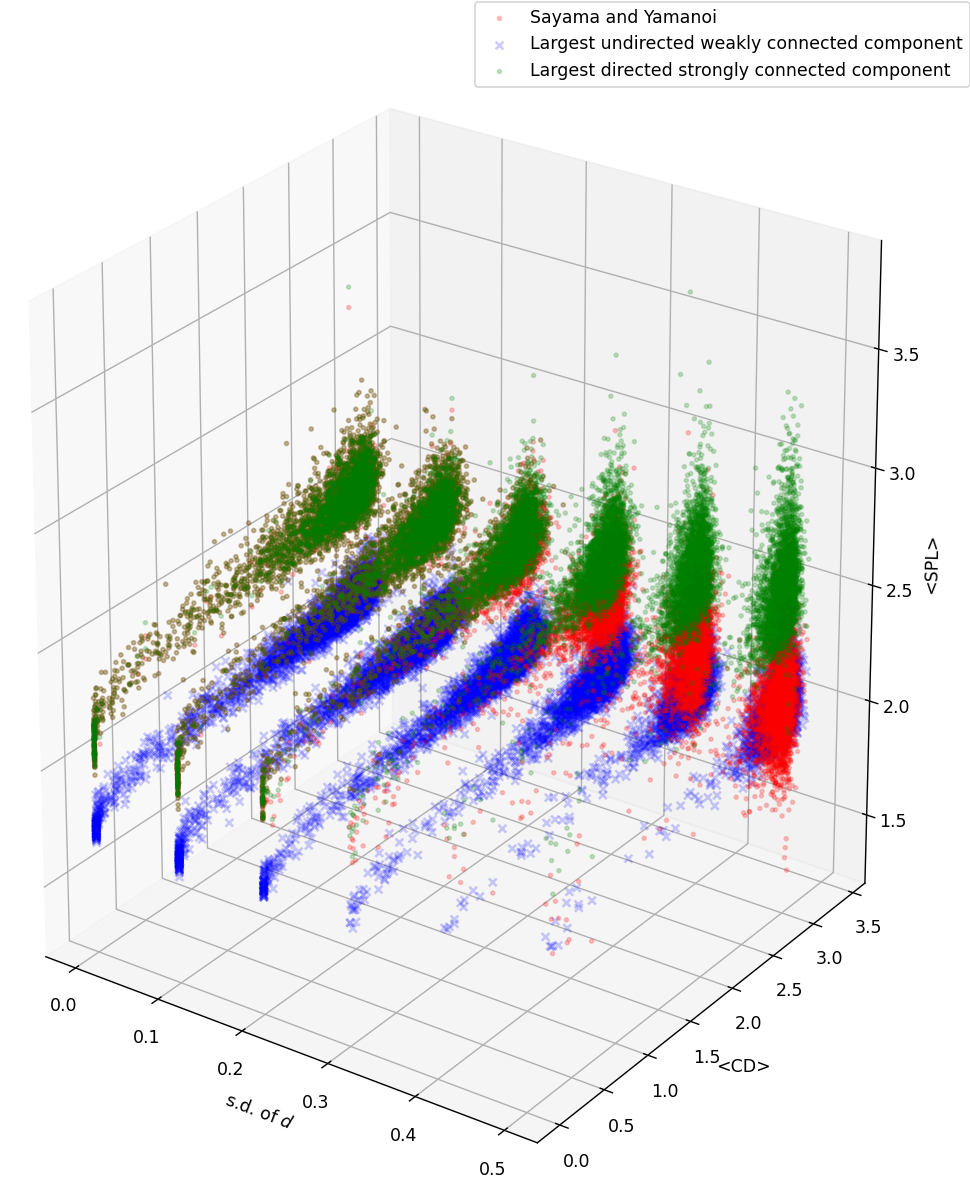
\includegraphics[width=.4\linewidth]{images/discrep view 1.png}}\hfill
    \subfloat[]{\label{View 2}
    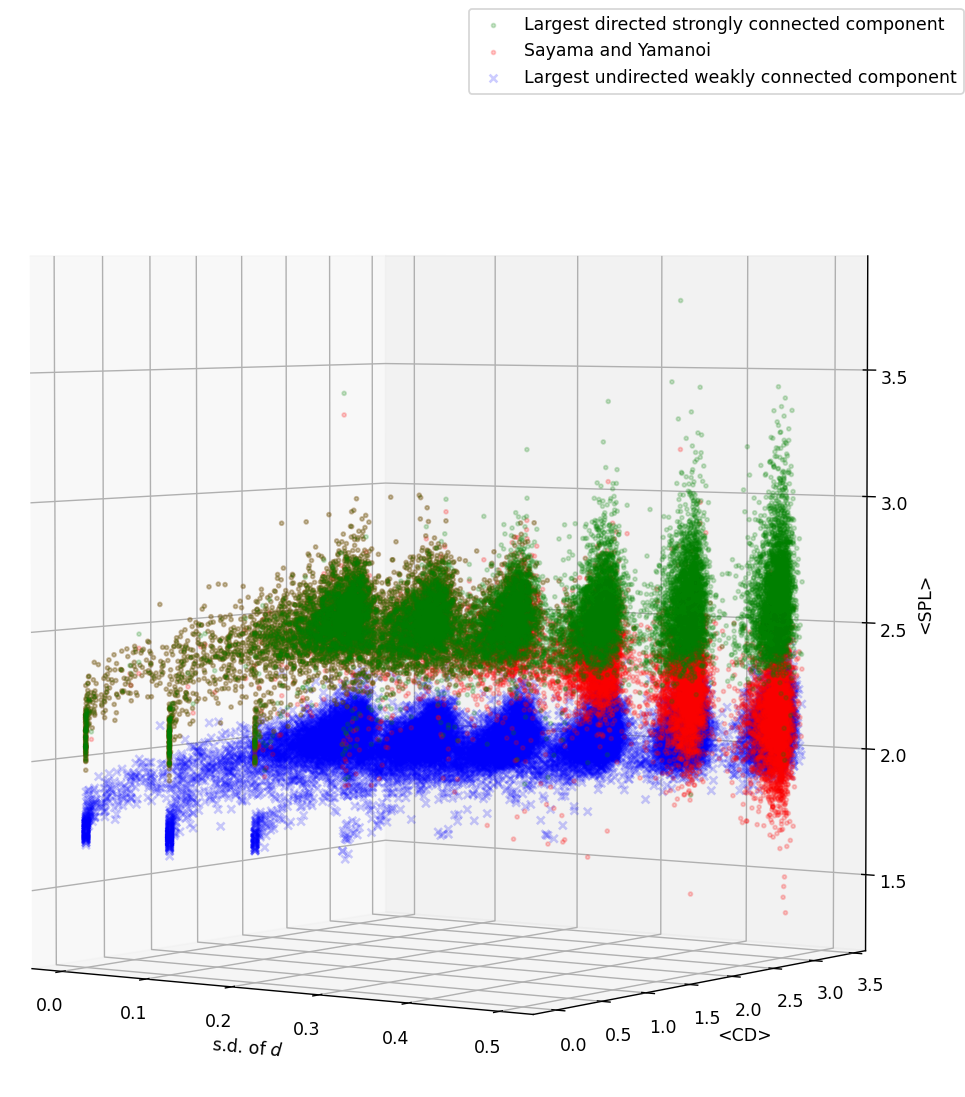
\includegraphics[width=.4\linewidth]{images/discrep view 2.png}}

    \caption{3D scatter plots showing CD, each
    standard deviation of $d$, and $SPL$ in red,
    $SPL_s$ in green, and $SPL_w$ in blue.}
    \label{figure}
\end{figure}


Figure 2 shows the same plot as done in the previous section, on the
same experiment data, except now
we have added $SPL_s$ and $SPL_w$.
Note that both $SPL_s$ and $SPL_w$ do not decrease as $\sd$ increases,
contrary to the trend of $SPL$.
However, the trend in CD remains similar.

\subsection{Component sizes}
\begin{figure}[hbt!]\centering
    \subfloat[]{\label{$\sd$ and $\sr$}
    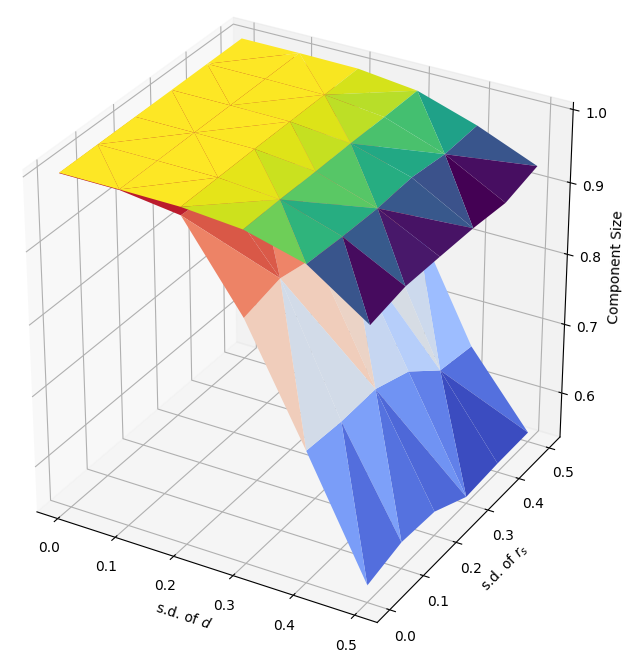
\includegraphics[width=.45\linewidth]{images/d - rs - compsize.png.png}}\par

    \subfloat[]{\label{$\sd$ and $\sw$}
    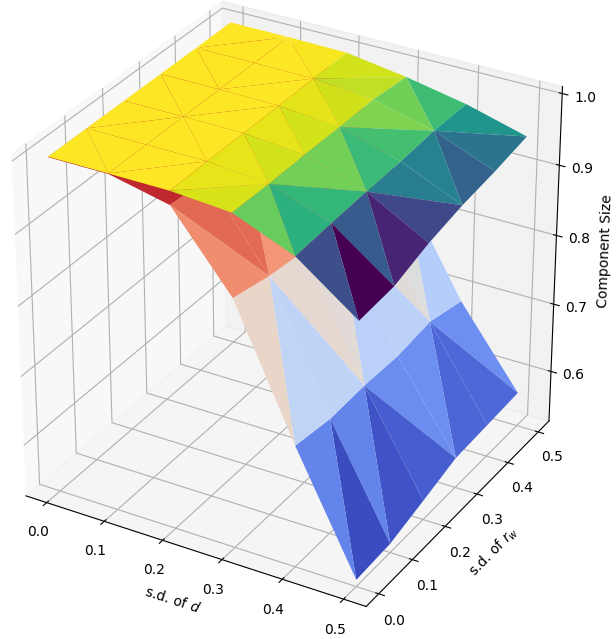
\includegraphics[width=.35\linewidth]{images/d-rw-compsize.png}}\hfill
    \subfloat[]{\label{$\sr$ and $\sw$}
    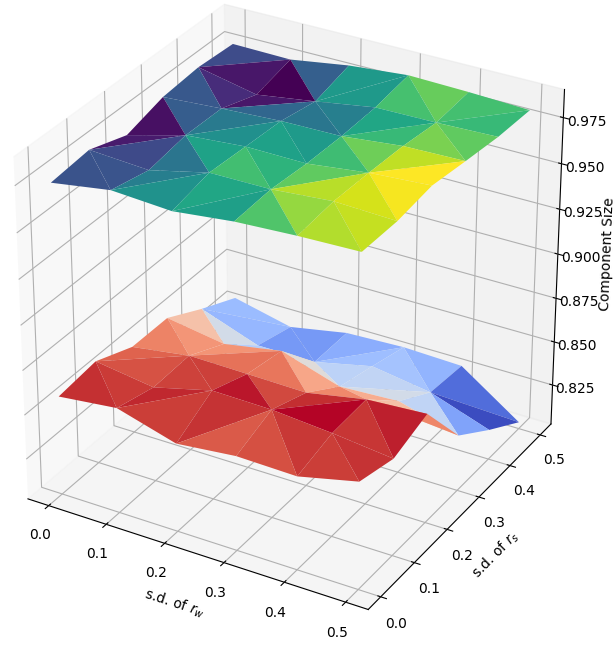
\includegraphics[width=.35\linewidth]{images/rw-rs-compsize.png}}

    \caption{3D surface plots showing the interactions between the diversities
    of combinations of $\sd$, $\sr$ and $\sw$ on the average size of the
    LSCC and WSCC (higher surface).}
    \label{figure}
\end{figure}
Figure 3 shows surface pltos of different combinations of the standard deviations
and the average LSCC and LWCC (higher surface) of all the trials for each pair of values.
We observe that these plots imply that $\sd$ have a large negative correlation
with the LSCC and LWCC.
The regression analysis on the average LSCC confirms this observation:

\begin{gather}\label{eq:base}
    |LSCC| ~ \thicksim ~ 1.04 - 0.40\sd - 0.01\sr - 0.02\sw -
                0.11\ds + 9,16\dw + 0.01\ssw \label{three}\\
\end{gather}

The resulting R-squared was 0.7 and all terms were extremely significant
according to the ANOVA analysis except for $\ssw$.
Note that in \ref{subsec:scwcreg}, we show that the size of the LSCC and LWCC
are highly correlated so we focus only on the LSCC.

\subsection{Definition of SPL}
From the two previous sections, we have seen that $SPL_s$ and $SPL_w$ do not
correlate with the trend of $SPL$ when $\sd$ increases.
We have also seen a trend that the networks become significantly less
strongly connected as $\sd$ increases.
Here we suspect that a nuance in the definition of SPL maybe the cause of this
discrepancy.

Notice that in the definition of SPL, the distance from node $u$ to $v$ is 0 when
$v$ is not reachable from $u$.
This is also reflected in the standard library algorithms for calculating
SPL in networkx.
The downward trend in $SPL$ can be explained by this fact and the fact that
the size of the LSCC decreases as $\sd$ increases.
As the size of the LSCC decreases, while the graph may remain connected,
less and less nodes are reachable from each other.
Therefore more and more pairs in the summation of the SPL calculation are 0.
Hence, we do not think that these experiments necessarily point to
increased structural connectivity as $\sd$ increases.
If it did, we would expect to also see a downward trend in $SPL_s$ and $SPL_w$.

Our position is that in the case of analyzing a connected, but not necessarily
strongly connected directed graph, the SPL metric does not make sense.
Even if many nodes are not reachable from each other, the SPL will still be
low and could even be below 1.
There is no way to distinguish between strong connectivity and high
fragmentation.

\subsection{Regression for SC vs WC} \label{subsec:scwcreg}

